\documentclass[a4paper,10pt, twocolumn]{article}
\usepackage[utf8]{inputenc}
\usepackage{amsmath}
\usepackage{amssymb}
\usepackage{amsthm}
\usepackage[usenames,dvipsnames]{color}
\usepackage{comment}
\usepackage{tikz}
\usepackage{verbatim}
\usetikzlibrary{arrows,shapes}
\usepackage{listings}
\usepackage{algorithm}
\usepackage{algpseudocode}
\usepackage{hyperref}
\usepackage{graphicx}
\usepackage{epstopdf}
\usepackage{enumitem}
\setlist{nolistsep}
\setlength{\parindent}{0cm}

%page boarders
\usepackage[top=3cm, bottom=3cm, left=2cm, right=2cm]{geometry}
\usepackage[style=numeric,backend=bibtex]{biblatex}
\addbibresource{../sources}
%\usepackage[style=mla,babel=hyphen,backend=biber]{biblatex}

\tikzstyle{vertex}=[circle,fill=black!25,minimum size=20pt,inner sep=0pt]
\tikzstyle{edge} = [draw,thick,->,>=latex,shorten >=1pt]
\tikzstyle{weight} = [font=\small]
\tikzstyle{selected edge} = [draw,line width=2pt,->,red!75,>=latex]
\tikzstyle{residual edge} = [draw,thick,->,blue!75,>=latex]
\tikzstyle{vertexE}=[circle,fill=black!25,minimum size=20pt,inner sep=0pt]

% Declare layers (for more convenience when drawing graphs)
\pgfdeclarelayer{background}
\pgfsetlayers{background,main}

\newtheorem{lemma}{Lemma}
\newtheorem{corollary}[lemma]{Corollary}
%\newtheorem{proof}[lemma]{Proof}

\title{Parallel Network Flow Algorithms \\ 
\large A follow up seminar to the Parallel Algorithms lecture\footnote{Jesper Larsson Träff, lecture "Parallel Algorithms", 2012 winter term at TU Wien}}
\author{Martin Kalany, 0825673}

\begin{document}
\maketitle

\section{Abstract}
\label{sec:abstract}

\section{Introduction}
\label{sec:intro}
\emph{Maximum flow problem}\footnote{Henceforth called \lstinline|MAX-FLOW| for brevity}


\section{Network flows}
\label{sec:networkFlows}
A \textbf{flow network} \cite{ahuja93} is given by $N = (G,s,t,c)$, where
\begin{itemize}
	\item $G =(V,E)$ is a directed graph
    \item $s$ and $t$, $s \neq t$ are the source and terminal node
   	\item $c:E\rightarrow \mathbb{R}_0^{+}$ assigns a capacity $\forall a \in E$
   	\item $n=\lvert V\rvert$, $m=\lvert E\rvert$
\end{itemize}

Furthermore, the following assumptions are made:
\begin{itemize}
	\item $G$ is connected
	\item $G$ is simple, i.e., does not contain loops or parallel arcs
	\item $\nexists P(s,t)$ with infinite capacity
\end{itemize}

\medskip
$f:E \rightarrow \mathbb{R}_0^{+}$ is a \textbf{flow} if it satisfies:
\begin{itemize}
	\item \emph{Capacity constraints:} $f(e) \leq c(e)$ $\forall e \in E$
	\item \emph{Flow conservation:} 
	$ \sum\limits_{v \in V} f(u,v) =  0 \Leftrightarrow IN(f,v) = OUT(f,v)$ $\forall v \in V \setminus \{s,t\}$
	\item \emph{Skew symmetry:} $f(v,w) = -f(w,v)$
	\item \emph{Value of a flow:} $\lvert f\rvert = f(V,t)$ 
\end{itemize}

A flow $f$
\begin{itemize}
	\item is a \emph{maximum flow} if $\lvert f\rvert \geq \lvert f'\rvert$, for any other flow $f'$
	\item \emph{saturates} an arc e if $f(e) = c(e)$
	\item is a \emph{maximal (or blocking) flow} if every directed path P(s,t) contains at least one saturated arc
\end{itemize}
\medskip
The \emph{residual capacity} of $e \in V \times V$ w.r.t. a flow $f$ is defined as $c_r(e) = c(e) - f(e)$. $G_r = (V, E_r)$ is the \emph{residual network}, where $E_r = \left\{e \in V \times V \lvert c_r(e) > 0\right\}$. A path $P$ from $s$ to $t$ in $G_r$ is called an \emph{augmenting path} and can be used to increase the flow $f$.

\section{Algorithm of Ford-Fulkerson}
\label{sec:fordfulkerson}

\section{Computitional Complexity}
\label{sec:cc}
The algorithmic complexity of the \emph{Ford-Fulkerson} algorithm is given as $O((n+m)*f_{max})$\footnote{$f_{max}$ is from here on used to denote the maximum flow} \cite{ahuja93,papa95}. This was improved by the \emph{Edmonds-Karp} algorithm to $O(n*m^2)$, by using shortest augmenting paths instead of arbitrarily chosen ones. Clearly, the \emph{maximum flow problem} can be solved in polynomial time with a sequential algorithm and is thus $\in P$.

Informally, algorithms may be \emph{efficiently parallelizeable} or \emph{inherently sequential}. The complexity class \textbf{NC} \cite{papa95} ("Nick's Class") contains all problems solvable in $O(log^{k_1}(n))$ time and $O(n^{k_2})$ total work. We give a useful alternate definition:  A language that is decided by PRAM in $O(log^{k_1}(n))$ time steps with $O(n^{k_2})$ processors available at each step is in $NC$. Problems $\in NC$ thus are solvable  in poly-logarithmic time requiring polynomial work (or resources). Problems $P \setminus NC$ are dubbed "inherently sequential", i.e., not parallelizeable efficiently. 

Clearly, $NC \subseteq P$, but whether $NC \subset P$ or $NC = P$ is still unknown. It follows that we do not know whether or not inherently sequential problems actually exist. The most likely problems to be hard to parallelize are P-complete problems. Since any problem $A \in P$ can be reduced to a P-complete problem $B$, a parallel algorithm that solves $B$ within poly-logarithmic time bounds would immediately imply that for all problems $\in P$ a parallel algorithm $\in NC$ exists \cite{papa95}.

As an example, the Ford-Fulkerson algorithm can not be parallelized trivially. Although constructing the residual network can be done in constant time $O(1)$ by assigning a processor to each edge $a \in E$ and augmenting paths can be found in $O(log^{2}n)$ time and $O(n^{2})$ work by a basic BFS search, the number of stages can not be reduced to less than $O(\sqrt(n))$ \cite{ahuja93}. Thus the total complexity, which is dominated by the number of stages, places the algorithm in $P \setminus NC$.
	
As shown in \cite{papa95}, \lstinline|MAX-FLOW| is P-complete and no parallel algorithm $\in NC$ is currently known for solving this problem. It is assumed that the problem is inherently sequential.

\section{Dinitz' scheme}
\label{sec:dinitz}
$N = (V,E,s,t,c)$ is a \textbf{layered network} \cite{yossi81} if each vertex $v \in V$ has a layer number $l(v)$ s.t.
\begin{itemize}
	\item $l(s) = 0$ and $0 \leq l(v) \leq l(t)$ $\forall v \in V$
	\item $(e = u \rightarrow v) \in E  \Rightarrow l(v) - l(u) = 1$
\end{itemize}
Figure \ref{fig:dinitz} shows a layered network and it's underlying directed acyclic network.

\begin{figure}
\begin{center}
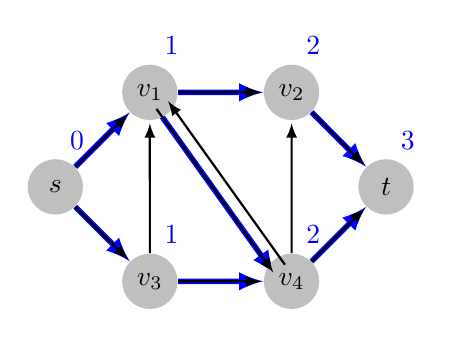
\begin{tikzpicture}[scale=1.2, auto,swap]
   	% draw the vertices
	\foreach \pos/\name/\layer in {{(0,2)/s/0}, {(1,3)/v_1/1}, {(2.5,3)/v_2/2},
    	                        {(1,1)/v_3/1}, {(2.5,1)/v_4/2}, {(3.5,2)/t/3}}
    \node[vertex,label={[color=blue]80:$\layer$}] (\name) at \pos {$\name$};
        
    %\node[vertex,label={[color=blue]80:$+12$}] (v_1) at (1.5,3) {$v_1$};
    % Connect vertices with edges and draw weights
    \foreach \source/ \dest in {s/v_1, s/v_3,v_3/v_1,
                                        v_1/v_2, v_4/v_2, v_3/v_4,
                                        v_2/t, v_4/t}
     \path[edge] (\source) -- (\dest);
        	
     %v_1/v_4/9
     \path[edge] ([xshift= -2pt, yshift= 5pt] v_4.center) -- ([xshift= 5pt, yshift= -2pt] v_1.center);
     \path[edge] ([xshift = 2pt, yshift= -5pt] v_1.center) -- ([xshift= -5pt, yshift= 2pt] v_4.center);
  
	% For convenience we use a background layer to highlight edges
    % This way we don't have to worry about the highlighting covering
	% weight labels. 
	\begin{pgfonlayer}{background}
    	\foreach \source /\dest in {s/v_3,v_2/t,s/v_1,v_1/v_2,v_3/v_4,v_4/t}
	      	\path[selected edge, color=blue] (\source) -- (\dest);		
	    \path[selected edge, color=blue] ([xshift = 2pt, yshift= -5pt] v_1.center) -- ([xshift= -5pt, yshift= 2pt] v_4.center);
	\end{pgfonlayer}
\end{tikzpicture}
\end{center}
\caption{A layered network (in blue) with layer numbers and it's underlying network}
\label{fig:dinitz}
\end{figure}

\begin{lemma}
\textbf{Dinitz' scheme} \cite{dinitz70} \\
A maximum flow problem in a general network can be transformed into $O(n)$ maximal flow problems in layered networks.
\end{lemma}

A layered network can easily be constructed from a directed acyclic network by performing breath-first search in  $O(log^{2}n)$ time. It follows that an algorithm that finds a maximal/blocking flow in a layered network can solve \lstinline|MAX-FLOW| in $O(n)$ iterations. The basic scheme is given in Algorithm \ref{algo:dinitz}

%TODO: remove comments?
\begin{algorithm}
\caption{Dinitz' scheme}
\label{algo:dinitz}
\begin{algorithmic}[1]
	\Function{MAX-FLOW}{$N=(V,E,s,t,c)$}
	\State start with some valid flow 
	\While{$l(t) \neq \infty$} \Comment{\textcolor{OliveGreen}{$O(n)$}}	
		\State Construct residual network $G_r$ \Comment{\textcolor{OliveGreen}{$O(n)$, $p=O(n)$}}
		\State Construct layered network $G_l$ from $G_r$ \Comment{\textcolor{OliveGreen}}{$O(m/p + n)$}
		\State $f_l$ = MAX-FLOW($G_l$)  \Comment{tbd}
		\State $f$ = $f$ + $f_l$ \Comment{\textcolor{OliveGreen}{$O(n)$}}
	\EndWhile
	\EndFunction
\end{algorithmic}
\end{algorithm}

\section{Algorithm of Shiloach and Vishkin}
\label{sec:shiloach}

\begin{algorithm}
\caption{Shiloach-Vishkin}
\label{algo:sv}
\begin{algorithmic}[1]
	\Function{MAX-FLOW}{$G_l$}
		\State EXCESS(s) = $\Sigma_{v \in L_1}$ c(s$\rightarrow$v)
		\State PUSH(s, EXCESS(s))
		\State i = 1
		\While{$\exists$ v $\in$ UNBALANCED}
			\State i++
			\If{$v$ is not blocked}
				\State PUSH(v, EXCESS(v))
			\EndIf
			\State RETURN(v, EXCESS(v))
		\EndWhile
	\EndFunction
\end{algorithmic}
\end{algorithm}

\begin{algorithm}
\caption{Shiloach-Vishkin: INITIALIZE}
\label{algo:sv_init}
At beginning of each pulse:	
\begin{algorithmic}[1]
	\Function{INTIALIZE}{v}
		\State \textcolor{blue}{P($e_j = v \rightarrow w$):}
		\State UPDATE($j$, $c_r(e_j)$) T-OUT(v)
		\State f($e_j$) = 0
		\State \textcolor{blue}{P(v):}
		\State head(v) = 0	
		\State k'(v) = 1	
 	\EndFunction
\end{algorithmic}
\end{algorithm}

\begin{algorithm}
\caption{Shiloach-Vishkin: PUSH}
\label{algo:sv_push}
$\forall v \in UNBALANCED$ do in parallel:
\begin{algorithmic}[1]
	\Function{PUSH}{v,EXCESS(v)}
		\State \textcolor{blue}{P(v):}
		\State $\alpha$ = min\{EXCESS(v), T-OUT(v)[root]\} 
		\State EXCESS(v) = EXCESS(v) - $\alpha$
		\State FIND($\alpha$, k, $\rho$) in T-OUT(v)
		\State \textcolor{blue}{P($e_j = v \rightarrow w$):}
		\If{k' $\leq$ j $\leq$ k}
 		\State UPDATE(j,1) in T-ACCESS(w)
		\State SUM(j,$S_j$) in T-ACCESS(w)
		\If{$j == k$}
			$q_j$ = $\rho$
		\Else
			\State $q_j$ = T-OUT(v)[1,j]
		\EndIf
		\State $f(e_j)$ = $f(e_j)$ + $q_j$
		\State TOTAL(w) = T-IN(w)[root]
		\State UPDATE(head(w) + $S_j$, $q_j$) in T-IN(w)
		\State UPDATE(j, T-OUT(v)[1,j] - $q_j$) in T-OUT(v)
		\State head(w) = head(w) + T-ACCESS(w)[root] 
		\State CLEAR(j) in T-ACCESS(w)
		\State EXCESS(w) = T-IN(w)[root] - TOTAL(w)
		\EndIf
		\State \textcolor{blue}{P(v):} k' = k
		\State \textcolor{blue}{P($e_d = v \rightarrow w$):}
		\If{EXCESS(v) $>$ 0}
			\State block v
		\EndIf
 	\EndFunction
\end{algorithmic}
\end{algorithm}


\begin{algorithm}
\caption{Shiloach-Vishkin: RETURN}
\label{algo:sv_return}
\begin{algorithmic}[1]
	\Function{RETURN}{v, EXCESS(v)}
		\State \textcolor{blue}{P(v):}
		\State FIND (T-IN(v)[root] - EXCESS(v), k, $\rho$) in T-IN(v)
		\State EXCESS(v) = 0
		\State \textcolor{blue}{$P(Q_j = (e_j = u \rightarrow v, q_j))$:}
		\State $d_j \rightarrow q_j$ for $k < j \leq head(v)$
		\State $d_j \rightarrow q_j - \rho$ if $j = k$
		\State UPDATE(j, 0) in T-IN(v) for $k < j \leq head(v)$
		\State UPDATE(j, $\rho$) in T-IN(v) if $j = k$
		\State UPDATE($r_j$,$d_j$) in T-EDGE($e_j$)
		\State $f(e_j)$ = $f(e_j)$ - T-EDGE($e_j$)[root]
		\State UPDATE($l_j$, T-EDGE($e_j$)[root] in T-SUM(u)
		\State EXCESS(u) = EXCESS(u) + T-SUM(u)[root]
		\State CLEAR($r_j$) in T-EDGE($e_j$)
		\State CLEAR($l_j$) in T-SUM(u)
		\State \textcolor{blue}{P(v):}
		\State head(v) = k
	\EndFunction
\end{algorithmic}
\end{algorithm}

\section{Algorithm of Goldberg and Tarjan}
\label{sec:goldberg}

\begin{algorithm}
\caption{Goldberg-Tarjan: INITIALIZE}
\label{algo:gt_init}
\begin{algorithmic}[1]
	\Function{INITIALIZE}{$N=(V,E,s,t,c)$}
	\ForAll{$e_i = (s,v_i) \in E$}
		\State create new atom $a_i$
		\State $size(a_i) = c(e_i)$
		\State $position(a_i) = v_i$
		\State $trace(a_i) = (s,v_i)$		
	\EndFor
	\EndFunction
\end{algorithmic}
\end{algorithm}

\begin{algorithm}
\caption{Goldberg-Tarjan: PUSH}
\label{algo:gt_push}
$\forall v \in V \setminus \{s,t\}$ and $v$ not blocked, do in parallel:
\begin{algorithmic}[1]
	\Function{PUSH}{$v$}
	\State Let $a_1 \dots a_k$ be atoms at vertex $v$
	\State Let $(v,w_1) \dots (v,w_l)$ be admissible arcs at $v$
	\State $\forall 1 \leq j \leq k: S(j) = \Sigma_{i=1}^{j} size(a_i)$
	\State $\forall 1 \leq j \leq l: R(j) = \Sigma_{i=1}^{j} c_r(v,w_i)$
	\State Assign $a_i$ to $(v, w_j)$:
	\If {$S(i) - size(a_i) \geq R(j) - c_r(v, w_j)$}
		\If{$S(i) \leq R(j)$}
			\State assign amount $size(a_i)$ of $a_i$ to $(v,w_j)$
		\Else
			\State assign amount $R(j)-S(i)+size(a_i)$ of $a_i$ to $(v,w_j)$
		\EndIf
	\EndIf
	\If {$S(i) - size(a_i) < R(j) - c_r(v, w_j)$}
		\If{$S(i) > R(j)$}
			\State assign amount $c_r(v,w_j)$ of $a_i$ to $(v,w_j)$
		\Else
			\State assign amount $S(i)-R(j)+c_r(v,w_j)$ of $a_i$ to $(v,w_j)$
		\EndIf
	\EndIf
	\If{$a_i$ assigned to more than 1 $(v,w_j)}$
		\ForAll{$(v,w_j)$ assigned to $a_i$}
			\If{assignment saturates $(v,w_j)$}
				\State create new atom $a_k$ 
				\State $size(a_k$) = quanta assigned to $(v,w_j)$
				\State $trace(a_k) = trace(a_i)$ 
				\State $position(a_k) = position(a_i)$
			\EndIf
		\EndFor
	\EndIf	
	\ForAll{$(v,w_j)$}
		\ForAll{$a_i \leftrightarrow (v,w_j)$}
			\State $f(v,w_j) = f(v,w_j) + size(a_i)$
			\State $location(a_i) = w_j$
			\State $trace(a_i) = trace(a_i) + w_j$
		\EndFor 
	\EndFor
	\If{$\forall (v,w_j):$ saturated}
		\State mark $v$ to block
	\EndIf	
	\State $\forall v_i$ marked to block: $block(v_i)$
	\ForAll{$w \in V$ and $w$ blocked}
		\ForAll{$a$ at $w$}
			\State Let $(v_a, w)$ be last arc on $trace(a)$
			\State $f(v_a, w) = f(v_a, w) - size(a)$
			\State $location(a) = v_a$
			\State $trace(a) = trace(a) - (v_a, w)$
		\EndFor
	\EndFor	
	\EndFunction
\end{algorithmic}
\bigskip
Repeat PUSH until all atoms arrive at $s$ or $t$
\end{algorithm}



\section{Further results}
\label{sec:further}

\section{bla}
text \cite{ahuja93} \cite{papa95} \cite{yossi81} \cite{vishkin92} \cite{goldberg89} \cite{goldberg91} \cite{goldberg98} \cite{johnson87} \cite{schieber89} \cite{cherivan89} 

%\pagebreak
\printbibliography
\end{document}
